\documentclass{article}
\usepackage{amsmath, enumerate, pgfplots, multicol, sfmath}
\pgfplotsset{compat = newest}
\usepackage[margin=0.5in]{geometry}
\renewcommand{\familydefault}{\sfdefault}
\raggedright
\pagestyle{empty}

\newcounter{pset}
\newcounter{key}

\title{Functions P-Set (ICM)}
\author{Bryan Bain}
\date{June 2022}

\begin{document}

\subsubsection*{Functions P-Set}

Given each of the following, find $f(-1)$, $f(0)$, and $f(2)$.
\begin{enumerate}
    \item $f(x) = -5x^2 + 6x - 10$
    \item \begin{tabular}{c|c|c|c|c|c}
        $\pmb{x}$ & $-2$ & $-1$ & 0 & 1 & 2 \\ \hline 
        $\pmb{f(x)}$ & 1 & 0 & $-2$ & 2 & $-1$ \\
    \end{tabular}
    \item \mbox{} \newline 
    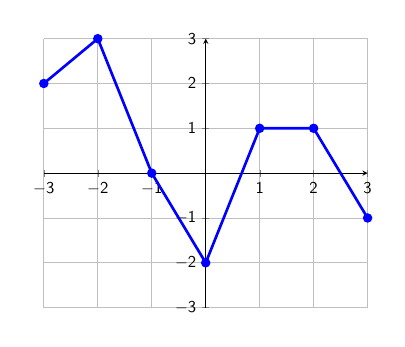
\begin{tikzpicture}[scale=0.6]
    \begin{axis}[
    axis lines = middle, xmin = -3, xmax = 3, ymin = -3, ymax = 3, xtick distance = 1, ytick distance = 1, grid
    ]
    \addplot[mark = *, blue, ultra thick] coordinates {
    (-3,2) (-2,3) (-1,0) (0,-2) (1,1) (2,1) (3,-1)
    };
    \end{axis}
    \end{tikzpicture}
\end{enumerate}     \setcounter{pset}{\value{enumi}}

Determine the domain of each. Write your answer using interval notation.
\begin{multicols}{4}
\begin{enumerate}   \setcounter{enumi}{\value{pset}}
    \item $f(x) = -10x$
    \item $g(x) = 3x^2 - 10$
    \item $h(x) = \sqrt{6 - x}$
    \item $j(x) = \frac{10x}{x^2-25}$
\end{enumerate}     \setcounter{pset}{\value{enumi}}
\end{multicols}
\begin{multicols}{4}
\begin{enumerate}   \setcounter{enumi}{\value{pset}}
    \item $k(x) = \frac{x-10}{5-x}$
    \item $m(x) = \sqrt{x^2+3}$
    \item $n(x) = \sqrt{x - 6}$
    \item $j(x) = \frac{x^2-36}{x-6}$
\end{enumerate}     \setcounter{pset}{\value{enumi}}
\end{multicols}

\vfill 

\dotfill \newline 
\texttt{Key:}
\begin{multicols}{2}
\begin{enumerate}   
    \item $f(-1) = -21, \, f(0) = -10, \, f(2) = -18$
    \item $f(-1) = 0, \, f(0) = -2, \, f(2) = -1$
\end{enumerate}     \setcounter{key}{\value{enumi}}
\end{multicols}
\begin{multicols}{2}
\begin{enumerate}   \setcounter{enumi}{\value{key}}
    \item $f(-1) = 0, \, f(0) = -2, \, f(2) = 1$ 
    \item $(-\infty, \infty)$
\end{enumerate} \setcounter{key}{\value{enumi}}
\end{multicols}
\begin{multicols}{2}
\begin{enumerate}   \setcounter{enumi}{\value{key}}
    \item $(-\infty, \infty)$ 
    \item $(-\infty, 6]$
\end{enumerate} \setcounter{key}{\value{enumi}}
\end{multicols}
\begin{multicols}{2}
\begin{enumerate}   \setcounter{enumi}{\value{key}}
    \item $(-\infty, -5) \cup (-5, 5) \cup (5, \infty)$ 
    \item $(-\infty, 5) \cup (5, \infty)$
\end{enumerate} \setcounter{key}{\value{enumi}}
\end{multicols}
\begin{multicols}{2}
\begin{enumerate}   \setcounter{enumi}{\value{key}}
    \item $(-\infty, \infty)$ 
    \item $[6, \infty)$
\end{enumerate} \setcounter{key}{\value{enumi}}
\end{multicols}
\begin{multicols}{2}
\begin{enumerate}   \setcounter{enumi}{\value{key}}
    \item $(-\infty, 6) \cup (6, \infty)$ 
\end{enumerate} \setcounter{key}{\value{enumi}}
\end{multicols}

\end{document}
